\documentclass[handout]{beamer}
\mode<presentation>
\usepackage{xcolor}
\usepackage[toc]{multitoc}
\usepackage{color}
\usepackage{graphicx}
\graphicspath{{../buku_ajar/buku_ajar_logika_matematika/figures/}}
\usepackage{tikz}
\usetikzlibrary{shapes,arrows,positioning,calc}
\usepackage{listings}
\usepackage{lmodern}
%\usepackage{enumitem}
\usetheme[secheader]{Boadilla}
\usecolortheme{whale}
\setbeamertemplate{caption}[numbered]
\setbeamertemplate{bibliography item}[text]
\setbeamertemplate{navigation symbols}{}

\theoremstyle{definition}
\newtheorem{definisi}[theorem]{Definisi}
\theoremstyle{example}
\newtheorem{contoh}[theorem]{Contoh}

\renewcommand*{\multicolumntoc}{2}

\setbeamertemplate{footline}
{
  \leavevmode%
  \hbox{%
  \begin{beamercolorbox}[wd=.333333\paperwidth,ht=2.25ex,dp=1ex,center]{author in head/foot}%
    \usebeamerfont{author in head/foot}\insertshortauthor%
  \end{beamercolorbox}%
  \begin{beamercolorbox}[wd=.433333\paperwidth,ht=2.25ex,dp=1ex,center]{title in head/foot}%
    \usebeamerfont{title in head/foot}\insertshorttitle
  \end{beamercolorbox}%
  \begin{beamercolorbox}[wd=.233333\paperwidth,ht=2.25ex,dp=1ex,right]{date in head/foot}%
    \usebeamerfont{date in head/foot}\insertshortdate{}\hspace*{2em} \insertframenumber{} / \inserttotalframenumber\hspace*{2ex} 
  \end{beamercolorbox}}%
  \vskip0pt%
}

\subtitle[Logika Matematika]{Logika Matematika}
\title[Landasan Teori dan Konsep Dasar]{Landasan Teori dan Konsep Dasar Logika Matematika}
\author{Cecep Suwanda, S.Si., M.Kom.}
\date{Maret 2025}
\institute{Universitas Bale Bandung}

\begin{document}

\maketitle

\section*{Daftar Isi}
\begin{frame}{Daftar Isi}
\frametitle{Daftar Isi}
\tableofcontents
\end{frame}

% ============================================================
% SECTION 2-1: Akar Filosofis
% ============================================================
\section{Akar Filosofis: Dari Silogisme hingga Logika Simbolik}

\begin{frame}
\frametitle{Landasan Logika Matematika}
\begin{itemize}
  \item Logika matematika merupakan instrumen untuk mengalihkan pernyataan bahasa alamiah yang mengandung ambiguitas menjadi rumus deterministik yang dapat diproses oleh mesin.
  \item Landasan ilmu komputer dirumuskan oleh para filsuf melalui gagasan \textbf{``Hukum Pasti Berpikir''}.
\end{itemize}
\end{frame}

\begin{frame}
\frametitle{Fajar Logika Yunani: Silogisme Aristoteles}
\begin{itemize}
  \item Pada rentang 384--322 SM, Aristoteles merintis \textbf{Silogisme}---struktur perdebatan menjadi rumus deduksi yang ketat.
  \item Keabsahan pernyataan dinilai berdasarkan \textit{struktur penalaran}, terlepas dari kebenaran faktual isi.
\end{itemize}
\begin{block}{Contoh Silogisme Klasik}
  \textbf{Premis Mayor:} Semua mamalia wajib mengembuskan karbon dioksida.\\
  \textbf{Premis Minor:} Seekor kucing perak tergolong bangsa mamalia.\\
  \textbf{Kesimpulan:} Kucing perak tersebut mengembuskan karbon dioksida.
\end{block}
\end{frame}

\begin{frame}
\frametitle{Era Revolusi Simbolik: George Boole}
\begin{itemize}
  \item \textbf{George Boole (1815--1864)}: matematikawan Inggris.
  \item Karya \textit{The Laws of Thought} (1854): nilai kebenaran direduksi menjadi rumus matematika.
  \item Memperkenalkan \textbf{Aljabar Boolean}---penalaran sebagai operasi biner 1 (True) dan 0 (False).
\end{itemize}
\end{frame}

\begin{frame}
\frametitle{Era Revolusi Simbolik: Gottlob Frege}
\begin{itemize}
  \item \textbf{Gottlob Frege (1879)}: karyanya \textit{Begriffsschrift} mengembangkan logika Boole.
  \item Memperkenalkan \textbf{Logika Predikat} dengan kuantifier:
  \begin{itemize}
    \item Universal ``Semua'' ($\forall$)
    \item Eksistensial ``Sebagian'' ($\exists$)
  \end{itemize}
  \item Dasar pencarian kondisi majemuk pada basis data relasional (SQL).
\end{itemize}
\end{frame}

\begin{frame}
\frametitle{Timeline Evolusi Logika Matematika}
\begin{center}
  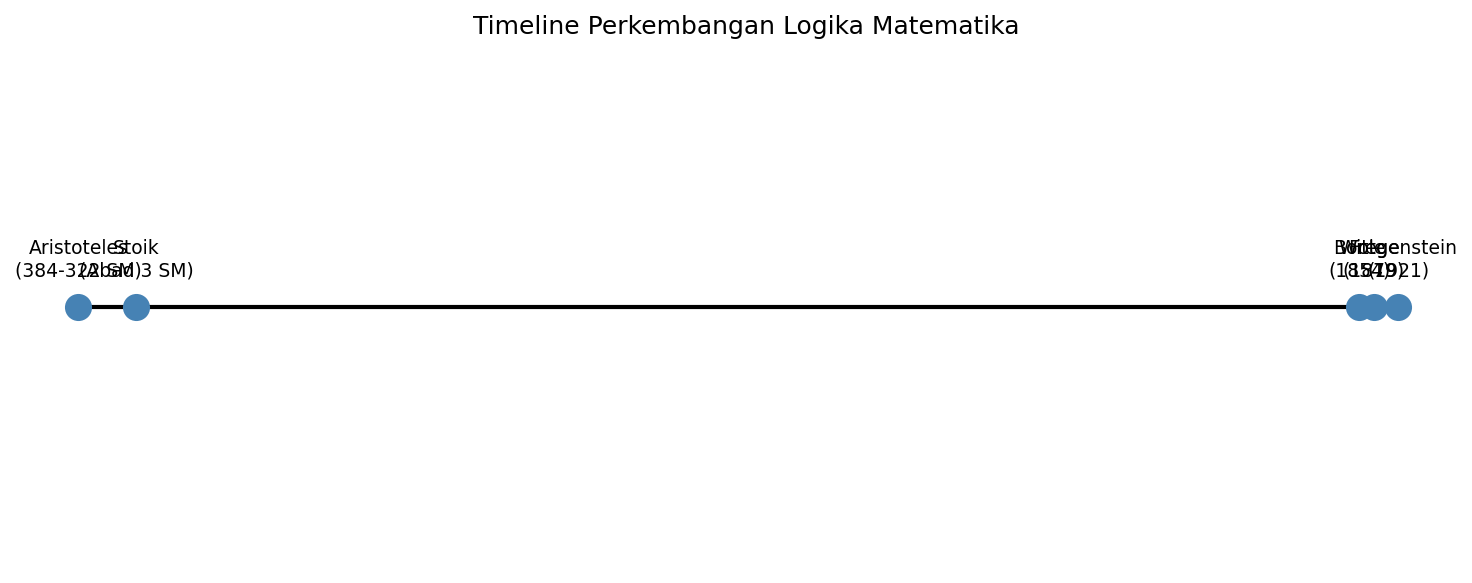
\includegraphics[width=0.9\textwidth]{timeline-logika}
\end{center}
\end{frame}

% ============================================================
% SECTION 2-2: Anatomi Argumen
% ============================================================
\section{Anatomi Argumen: Premis, Konklusi, dan Validitas}

\begin{frame}
\frametitle{Komponen Pembangun Argumen Formal}
\begin{table}
\small
\begin{tabular}{|l|p{8cm}|}
\hline
\textbf{Terminologi} & \textbf{Anatomi Fungsional} \\
\hline
\textbf{Proposisi} & Satuan terkecil kalimat asertif; bernilai BENAR (T) atau SALAH (F). \\
\hline
\textbf{Premis} & Kumpulan hipotesis yang diasumsikan benar di awal. \\
\hline
\textbf{Kesimpulan} & Hasil penerapan aturan inferensi terhadap premis. \\
\hline
\textbf{Aturan Inferensi} & Aturan yang memverifikasi langkah dari premis menuju kesimpulan. \\
\hline
\end{tabular}
\end{table}
\end{frame}

\begin{frame}
\frametitle{Visualisasi Alur Argumen}
\begin{center}
\begin{tikzpicture}[
  node distance=0.8cm,
  premis/.style={rectangle, draw=black, fill=blue!15, rounded corners, minimum width=2.2cm, minimum height=0.6cm, font=\small\bfseries},
  inferensi/.style={rectangle, draw=black, fill=green!15, rounded corners, text width=2.5cm, minimum height=0.8cm, align=center, font=\small\bfseries},
  kesimpulan/.style={rectangle, draw=black, fill=orange!15, rounded corners, text width=1.8cm, minimum height=0.6cm, align=center, font=\small\bfseries},
  arrow/.style={->, thick, >=stealth}
]
  \node[premis] (p1) {Premis 1};
  \node[premis, below=of p1] (p2) {Premis 2};
  \node[inferensi, right=1.8cm of $(p1)!0.5!(p2)$] (inf) {Aturan Inferensi};
  \node[kesimpulan, right=1.8cm of inf] (k) {Konklusi};
  \draw[arrow] (p1.east) -- (inf.west);
  \draw[arrow] (p2.east) -- (inf.west);
  \draw[arrow] (inf.east) -- (k.west);
\end{tikzpicture}
\end{center}
\end{frame}

\begin{frame}
\frametitle{Validitas vs Kebenaran Faktual}
\begin{definisi}[Hukum Absolut Argumen Valid]
Argumen dinyatakan \textbf{valid} apabila struktur sintaksnya menjamin: jika semua premis diasumsikan Benar (T), maka tidak mungkin kesimpulan bernilai Salah (F).\\
Validitas ditentukan dari ketepatan jalur inferensi, \textbf{bukan} dari kebenaran material premis.
\end{definisi}
\end{frame}

\begin{frame}
\frametitle{Contoh: Argumen Valid Secara Struktur}
\begin{contoh}
\textbf{Premis 1:} Jika Budi makan durian, maka Budi melahirkan alien.\\
\textbf{Premis 2:} Budi sedang makan durian.\\
\textbf{Kesimpulan:} Budi melahirkan alien.\\
\vspace{0.3cm}
\textbf{Penilaian: Argumen valid secara struktur.}\\
Meskipun kesimpulan tidak sesuai fakta empiris, struktur \textit{Modus Ponens} bekerja sesuai ketentuan.
\end{contoh}
\end{frame}

\begin{frame}
\frametitle{Contoh: Argumen Invalid---Fallacy}
\begin{contoh}[Fallacy of Affirming the Consequent]
\textbf{Premis 1:} Jika badai halilintar turun, maka stasiun TV mati.\\
\textbf{Premis 2:} Stasiun TV mati.\\
\textbf{Kesimpulan:} Badai halilintar turun.\\
\vspace{0.3cm}
\textbf{Penilaian: Argumen invalid.}\\
Stasiun TV dapat mati karena sebab lain (kerusakan peralatan). Aturan inferensinya tidak sesuai.
\end{contoh}
\end{frame}

% ============================================================
% SECTION 2-3: Logika Boolean & Perangkat Lunak
% ============================================================
\section{Logika Boolean dalam Arsitektur Perangkat Lunak}

\begin{frame}
\frametitle{Boolean sebagai Dasar Control Flow}
\begin{itemize}
  \item Struktur \texttt{IF}, \texttt{ELSE IF}, \texttt{WHILE} ditentukan oleh evaluasi ekspresi Boolean (True/False).
  \item Tanpa evaluasi kondisi logika, program hanya mengeksekusi pernyataan secara berurutan tanpa percabangan.
\end{itemize}
\end{frame}

\begin{frame}
\frametitle{Visualisasi Keputusan Bercabang}
\begin{center}
\begin{tikzpicture}[
  node distance=0.6cm,
  decision/.style={diamond, draw=black, fill=red!15, aspect=2, align=center, font=\small\bfseries, text width=2cm},
  process/.style={rectangle, draw=black, fill=blue!15, rounded corners, minimum height=0.6cm, text width=2.2cm, align=center, font=\small},
  start/.style={ellipse, draw=black, fill=green!20, font=\small\bfseries},
  arrow/.style={->, thick, >=stealth}
]
  \node[start] (start) {Mulai};
  \node[decision, below=of start] (cond) {Kondisi Boolean?};
  \node[process, below left=0.8cm and 0.8cm of cond] (t) {Cabang True};
  \node[process, below right=0.8cm and 0.8cm of cond] (f) {Cabang False};
  \node[process, below=2.2cm of cond] (end) {Penyatuan Alur};
  \draw[arrow] (start) -- (cond);
  \draw[arrow] (cond) -| node[near start, left, font=\bfseries\small, text=blue] {T} (t);
  \draw[arrow] (cond) -| node[near start, right, font=\bfseries\small, text=red] {F} (f);
  \draw[arrow] (t) |- (end);
  \draw[arrow] (f) |- (end);
\end{tikzpicture}
\end{center}
\end{frame}

\begin{frame}[fragile]
\frametitle{Operator AND, OR, NOT dalam Kode}
\begin{block}{Contoh: Filter Keamanan Finansial}
Akses diberikan jika: (IP domestik ATAU staf VIP) DAN usia tidak balita.
\end{block}
\begin{lstlisting}[basicstyle=\ttfamily\scriptsize, frame=single,
  breaklines=true, breakatwhitespace=true, columns=fullflexible,
  linewidth=0.92\linewidth]
ip_domestik = True
staf_vip = False
usia_akun_tahun = 3

izin_lolos = (ip_domestik or staf_vip) and not (usia_akun_tahun < 12)
# Hasil: (True or False) and not False
#        = True
\end{lstlisting}
\end{frame}

% ============================================================
% SECTION 2-4: AI & Basis Data
% ============================================================
\section{Fondasi AI dan Basis Data Relasional}

\begin{frame}
\frametitle{Aljabar Relasional dan SQL}
\begin{itemize}
  \item Aljabar Relasional merupakan turunan dari operasi Konjungsi (AND), Disjungsi (OR), dan kuantifikasi predikat.
  \item Data diproses melalui \textbf{Aljabar Relasional}---bukan manual.
\end{itemize}
\end{frame}

\begin{frame}[fragile]
\frametitle{Contoh Klausa WHERE dalam SQL}
\begin{lstlisting}[language=SQL, basicstyle=\ttfamily\scriptsize, frame=single,
  breaklines=true, breakatwhitespace=true, columns=fullflexible,
  linewidth=0.92\linewidth]
SELECT nama_lengkap, nim 
FROM Tabel_Mahasiswa_Nasional
WHERE (fakultas = 'MIPA') 
  AND (usia_tahun < 30) 
  AND NOT (status_skorsing 
    = 'Kriminal');
\end{lstlisting}
\begin{block}{}
Struktur kurung serta operator \texttt{AND}, \texttt{OR}, \texttt{NOT} memastikan presisi basis data.
\end{block}
\end{frame}

\begin{frame}
\frametitle{Rules Engine pada Sistem Pakar AI}
\begin{itemize}
  \item \textit{Expert Systems} menggunakan \textit{Knowledge-based System Reasoning Engine}.
  \item Sistem pakar medis bekerja menurunkan deduksi \textit{Modus Ponens} dari kumpulan fakta.
\end{itemize}
\begin{block}{Contoh Aturan WHO}
\textbf{Aturan 1:} JIKA Pasien punya suhu $> 39^\circ$C DAN bercak kulit MAKA diagnosis Cacar Akut.\\
\textbf{Aturan 2:} JIKA Cacar Akut DAN usia $< 5$ tahun MAKA prioritas Karantina ICU.
\end{block}
\end{frame}

% ============================================================
% SECTION 2-5: Gerbang Sirkuit
% ============================================================
\section{Gerbang Sirkuit Digital}

\begin{frame}
\frametitle{Transistor dan Gerbang Logika}
\begin{itemize}
  \item Transistor menerjemahkan nilai Boolean 1/0 menjadi tegangan listrik (tinggi/rendah).
  \item \textit{Logic Gates} mengimplementasikan operasi AND, OR, NOT.
\end{itemize}
\begin{block}{Gerbang Dasar}
  \textbf{AND:} Output 1 hanya bila kedua input 1.\\
  \textbf{OR:} Output 1 bila minimal satu input 1.\\
  \textbf{NOT:} Output membalik nilai input.
\end{block}
\end{frame}

\begin{frame}
\frametitle{Simbol Gerbang Logika}
\begin{center}
  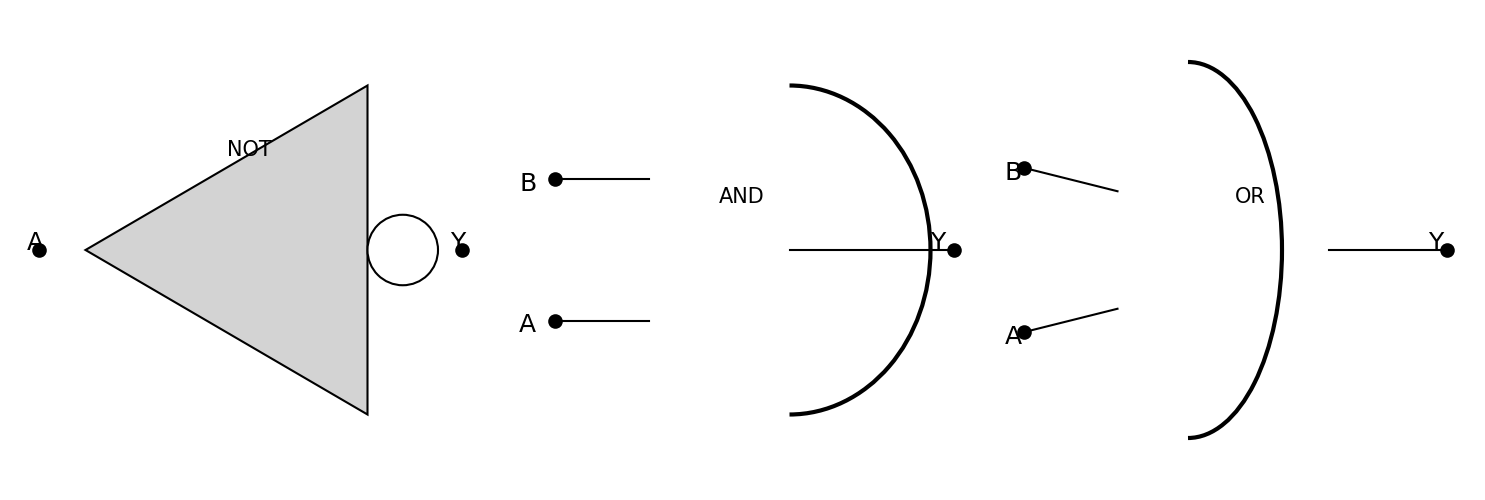
\includegraphics[width=0.85\textwidth]{logic-gates}
\end{center}
\end{frame}

\begin{frame}
\frametitle{Optimasi Rangkaian dengan Aljabar Boolean}
\begin{block}{Spesifikasi Awal}
$Y = (A \land B) \lor (A \land \neg B)$ --- memerlukan 2 AND, 1 NOT, 1 OR.
\end{block}
\begin{block}{Penyederhanaan}
$Y = A \land (B \lor \neg B) \equiv A \land \text{True} \equiv \textbf{A}$\\
Rangkaian hanya memerlukan satu kabel dari input A ke output Y. Biaya material berkurang signifikan.
\end{block}
\end{frame}

% ============================================================
% SECTION 2-6: Peta Jalur Materi
% ============================================================
\section{Peta Jalur Materi}

\begin{frame}
\frametitle{Taksonomi Buku Ajar}
\begin{center}
\begin{tikzpicture}[
  node distance=0.5cm and 0.8cm,
  box/.style={rectangle, draw=black, rounded corners, fill=blue!10, text width=2cm, minimum height=0.6cm, align=center, font=\scriptsize},
  root/.style={rectangle, draw=black, rounded corners, fill=green!20, text width=2.8cm, minimum height=0.7cm, align=center, font=\scriptsize\bfseries},
  arrow/.style={->, thick, >=stealth}
]
  \node[root] (root) {Fondasi Logika Matematika};
  \node[box, below left=1cm and 0.3cm of root] (b3) {Bab 3--4\\Proposisional};
  \node[box, below=1cm of root] (b4) {Bab 5--6\\Inferensi};
  \node[box, below right=1cm and 0.3cm of root] (b5) {Bab 7--8\\Predikat};
  \node[box, below=1.5cm of b4] (b6) {Bab 9--10\\Induksi \& Rekursi};
  \draw[arrow] (root) -- (b3);
  \draw[arrow] (root) -- (b4);
  \draw[arrow] (root) -- (b5);
  \draw[arrow] (b3) -- (b4);
  \draw[arrow] (b4) -- (b5);
  \draw[arrow] (b5) -- (b6);
  \draw[arrow] (b4) -- (b6);
\end{tikzpicture}
\end{center}
\end{frame}

\begin{frame}
\frametitle{Ringkasan Peta Materi}
\begin{itemize}
  \item \textbf{Bab 3--4:} Logika Proposisional, ekuivalensi, tautologi, tabel kebenaran.
  \item \textbf{Bab 5--6:} Modus Ponens, Modus Tollens, pembuktian langsung, kontradiksi, kontraposisi.
  \item \textbf{Bab 7--8:} Logika Predikat ($\forall$/$\exists$), kueri basis data, sistem pakar.
  \item \textbf{Bab 9--10:} Induksi Matematika, rekursi, validasi algoritma.
\end{itemize}
\end{frame}

% ============================================================
% RANGKUMAN
% ============================================================
\section{Rangkuman}

\begin{frame}
\frametitle{Rangkuman}
\begin{itemize}
  \item Logika bermula dari Silogisme Aristoteles, dikembangkan Boole (Aljabar Boolean) dan Frege (Logika Predikat).
  \item \textbf{Validitas} memisahkan kebenaran faktual dengan keabsahan struktur inferensi.
  \item Percabangan \texttt{IF--ELSE} di perangkat lunak menggunakan prinsip Boolean.
  \item Logika predikat menjadi dasar SQL dan mesin inferensi AI.
  \item Gerbang logika (AND, OR, NOT) menerjemahkan hukum Boolean ke sirkuit silikon. Penyederhanaan ekspresi mengurangi biaya produksi.
\end{itemize}
\end{frame}

\begin{frame}
\frametitle{Kata Kunci}
\begin{center}
Silogisme Aristotelian $\bullet$ Aljabar Boolean $\bullet$ Anatomi Argumen\\
Validitas Struktural $\bullet$ Control Flow $\bullet$ Gerbang Logika $\bullet$ Aljabar Relasional
\end{center}
\end{frame}

\end{document}
